\section{Resultados y conclusiones}


\subsection{Impresiones en pantalla y entrega del sistema}

\begin{figure}[htb]
\begin{center}
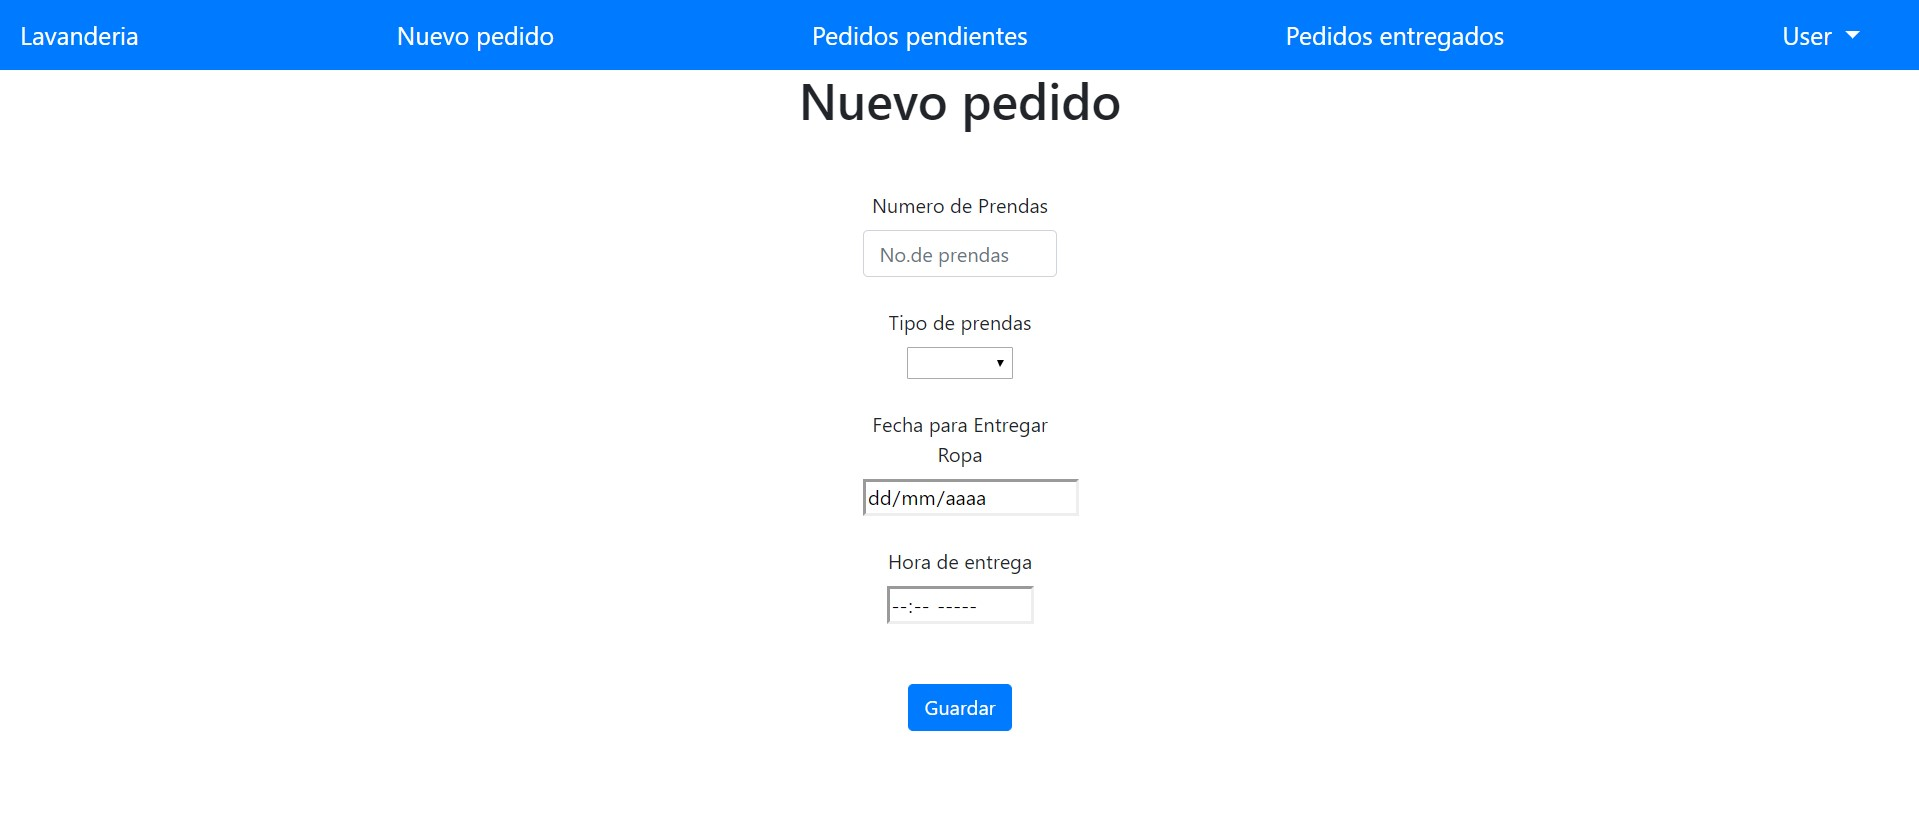
\includegraphics[width=12cm]{./imagenes/nuevopedido.jpg}
\end{center}
\caption{Moduló de pedido nuevo -cliente}
\end{figure}


\begin{figure}[htb]
\begin{center}
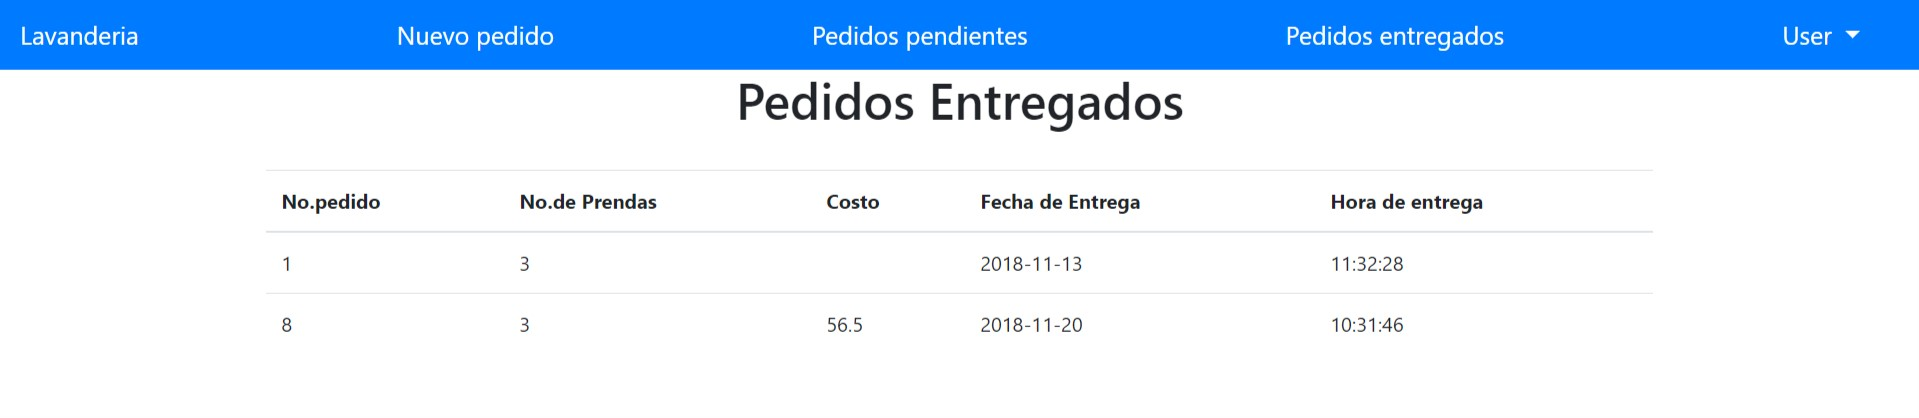
\includegraphics[width=12cm]{./imagenes/pedidosentregadoscliente.jpg}
\end{center}
\caption{Moduló de pedidos entregados -cliente}
\end{figure}

\begin{figure}[htb]
\begin{center}
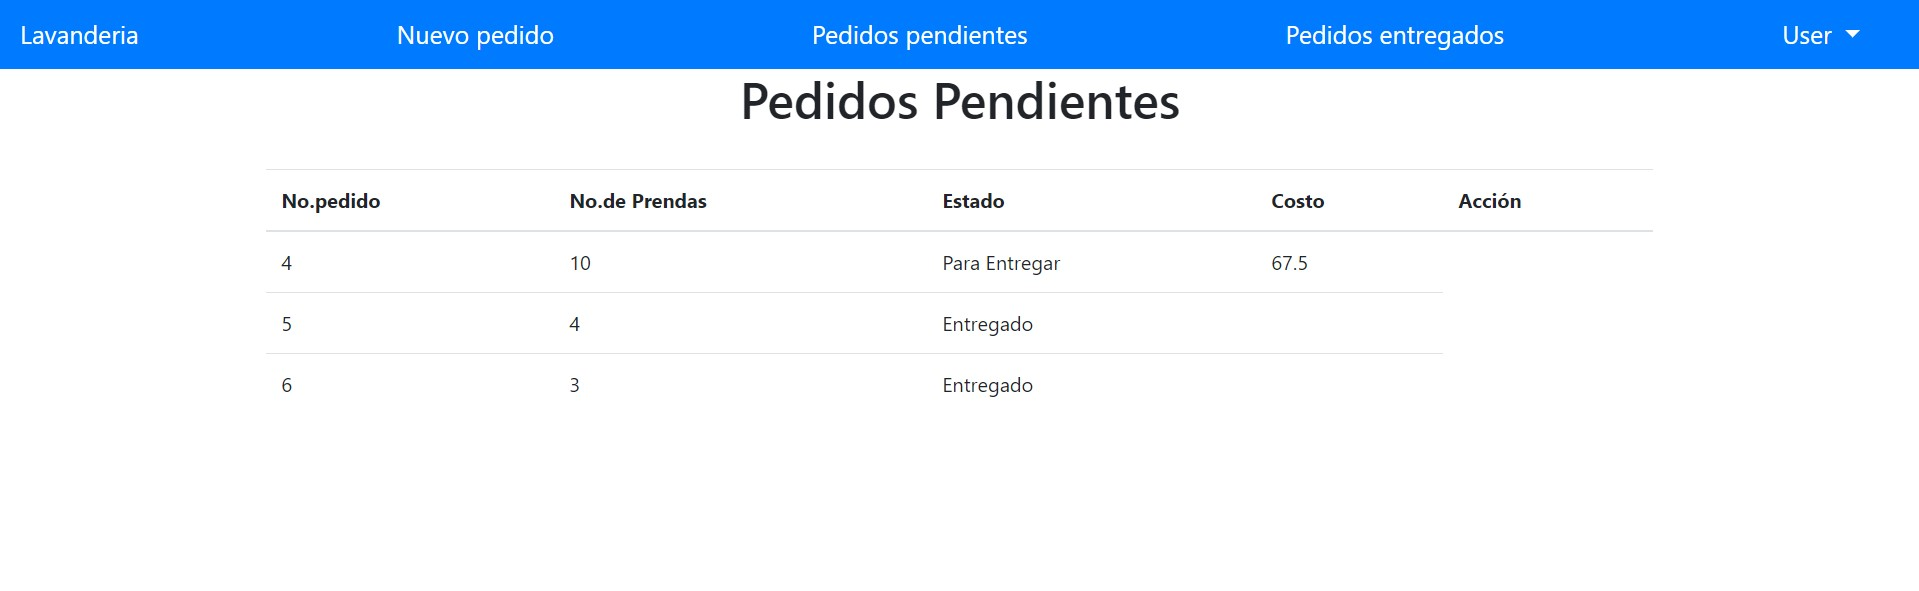
\includegraphics[width=12cm]{./imagenes/pedidospendientescliente.jpg}
\end{center}
\caption{Moduló de pedidos pendientes -cliente}
\end{figure}

\newpage


%admin fotos


\begin{figure}[htb]
\begin{center}
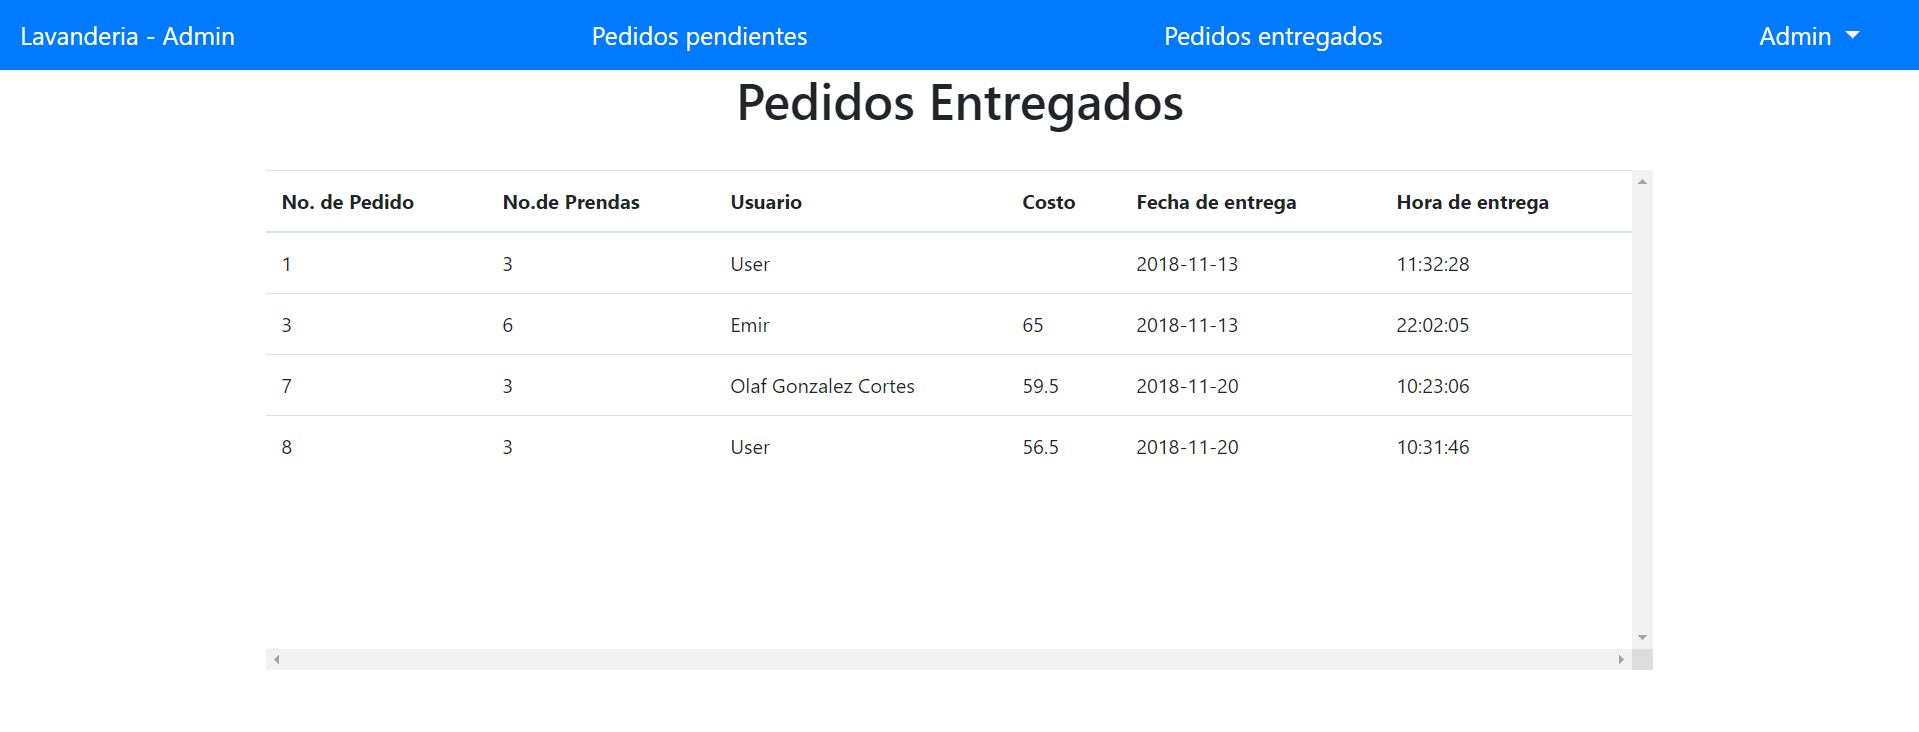
\includegraphics[width=12cm]{./imagenes/pedidosentregadosadmin.jpg}
\end{center}
\caption{Moduló de pedidos entregados -admin}
\end{figure}


\begin{figure}[htb]
\begin{center}
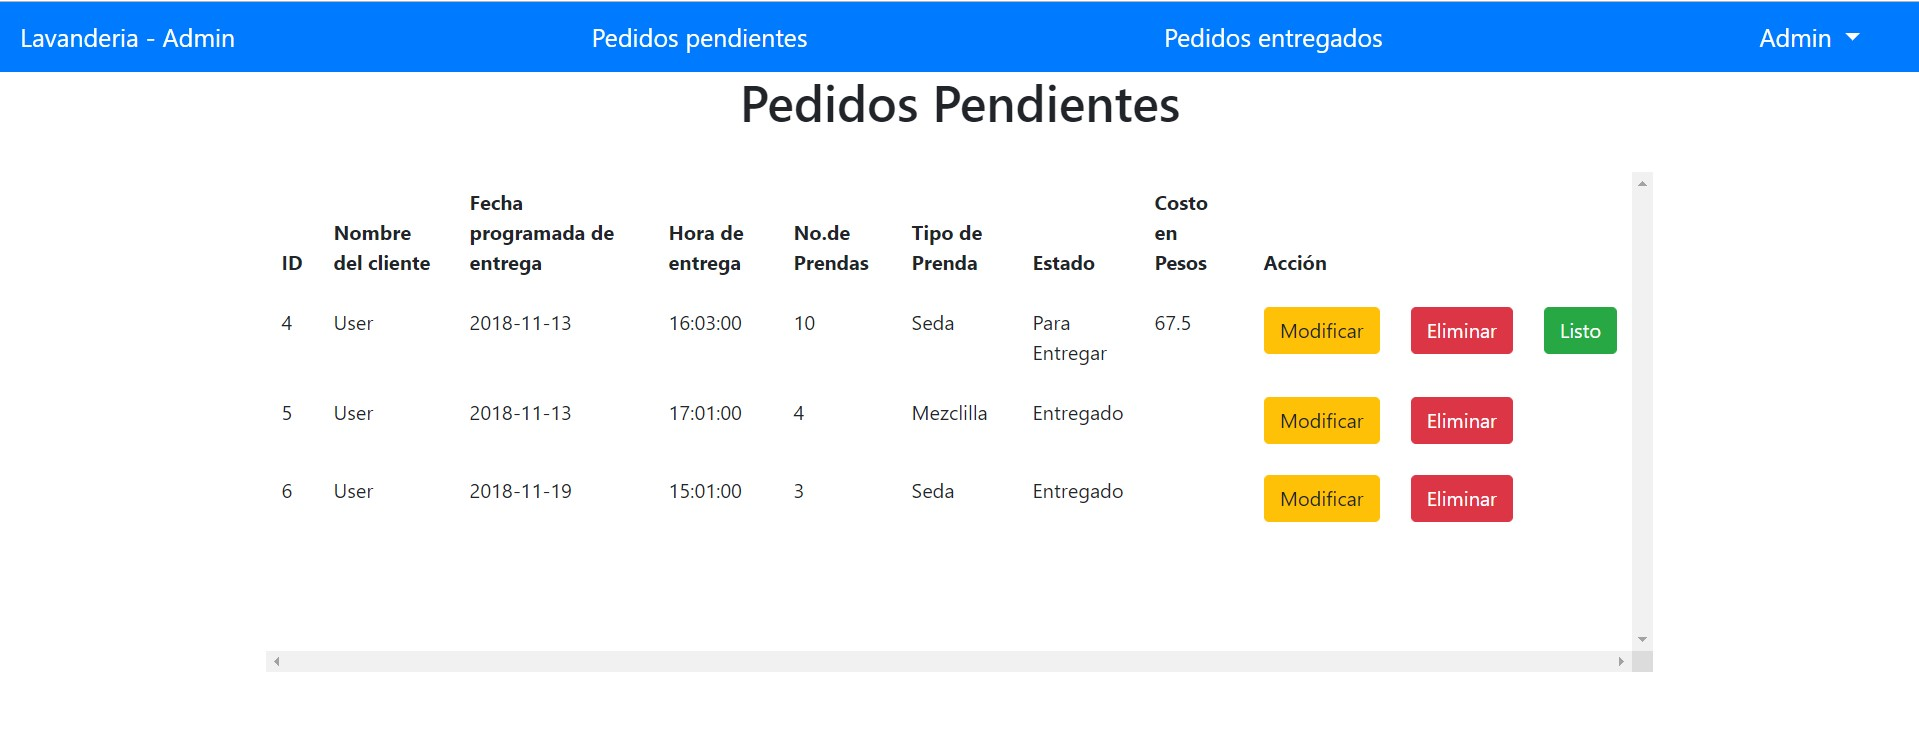
\includegraphics[width=12cm]{./imagenes/pedidospendientesadmin.jpg}
\end{center}
\caption{Moduló de pedidos pendientes -admin}
\end{figure}


\section{Conclusión individual por cada integrante del equipo}
\textbf{Emir}: Sin duda alguna el software tiene un papel importante para la innovación de las tareas que realizamos día con día y nuestra carrera se encarga de llevar todo el proceso de su desarrollo desde el análisis hasta la codificación y mantenimiento, durante todo ese proceso hay muchas herramientas que pueden ser de gran ayuda como son Frameworks, lenguajes de programación, normas y estándares de calidad, diagramas UML entre otras, si se le da un buen uso.

\textbf{Olaf}: El desarrollo de este sitio a ampliado la forma en la que investigo y programo, ya que este framework ha hecho que la programación sea mucho más sencilla y efectiva.

\section{Trabajos a fututo}
Al sitio web que desarrollamos se pueden agregar módulos que trabajen en conjunto para una mejor automatización, como puede ser una sección de ayuda para mostrarle a los clientes los servicios que ofrecen y como utilizar el sitio, información sobre el local e indicaciones de cómo llegar en Google Maps, si el negocio de nuestro cliente crece puede incluso hacer entregas a domicilio y ofrecerle al cliente una sección para el seguimiento de sus pedidos en tiempo real.


